\documentclass{article}

\usepackage[hidelinks]{hyperref}
\usepackage{enumitem}
\usepackage{amsfonts}
\usepackage[framemethod = tikz]{mdframed}

\usepackage{geometry}
\geometry{
	a4paper,
	top=3cm,
	bottom=3cm,
	left=2.5cm,
	right=2.5cm,
	heightrounded,
	bindingoffset=0mm
}

\hypersetup{
	colorlinks=false,
	linkcolor=blue,
	filecolor=magenta,
	urlcolor=cyan,
	linktocpage=false
}

\usepackage{listings}
\usepackage{titlesec}

\newcommand\chaptername{Section}
\titleformat{\section}[display]{\normalfont\huge\bfseries}{\chaptername\ \thesection}{20pt}{\Huge}
\titlespacing*{\section}{0pt}{50pt}{40pt}
\newcommand\sectionbreak{\clearpage}

\title{ 
	
\includegraphics[width=95mm]{img/PolimiLogo.png} \\
	\bigskip
	Design Document (DD)
}

\author{
	Davide Rossetto 894029, Alessandro Tatti 883861
}

\date{
	Delivery date: 2017 Nov 26\\
	\bigskip v0.4
}

\begin{document}
	
\maketitle
\newpage
\tableofcontents
\newpage
	
	
	\section{Introduction}
	

	
	\subsection{Purpose}
	The structure of the following document is divided into two sections:
	\begin{enumerate}
	\item Design Document (main section)
	\item Integration Test Plan Document (secondary section)
	\end{enumerate}

	\bigskip
	The Design Document (DD) is intended to provide a more detailed functional description of the Travlendar + system – to - be by providing technical details and describing the main architectural components, their interfaces, and their interactions.
	
	The relationships among the different modules are highlighted using UML standards and other useful diagrams that show the structure of the system.
	
	The document has to guide the software development team to implement the project architecture, providing a stable reference and a unique view of all parts of the software, defining their operation.

	\bigskip
	The second part of the document is intended to provide guidelines to adequately carry out the planning of the integration test phase.
	
	The document includes determining which necessary tools, drivers and data structures that will be useful during the test process.

	
	
	\subsection{Scope}
	The system aims to support a personal event management service, providing features for choosing the best path, means of transport, and insertion of the break. The system must also make sure there are no overlap among events and among events and pauses.

	The system is structured with a four-layer architecture. The purpose of the document is to describe this architecture in detail.

	\bigskip
	The system described is suitable for different types of customers: different actors that interact with the system - to – be by generating a client-server dualism, so the flow of requests and responses.
	
	The architecture must be designed with the intention of being maintainable and extensible, to make future possible changes.
	
	\bigskip
	This document aims to guide the implementation phase so that cohesion and decoupling are increased as much as possible. In order to do this, individual components must not include too many independent functions and reduce interdependence.
	
	This document will follow specific architectural styles and design templates used for future implementation, as well as common design paradigms that combine useful features of this concepts.


	
	\subsection{Definitions, Acronyms, Abbreviations}
	\begin{description}
	\item[ACID:] Atomicity, Consistency, Isolation and Durability. This is the set of properties of database transactions.
	\item[DD:] Design Document.
	\item[DBMS:] DataBase Management System.
	\item[E-R diagram:] entity – relationship diagram
	\item[ITPD:] Integration Test Plan Document.
	\item[JPA:] Java Persistence API.
	\item[MVC:] Model-View-Controller.
	\item[RASD:] Requirements Analysis and Specification Document.
	\item[UML:] Unified Modeling Language
	\item[UX:] User Experience.
	\end{description}
	
	
	\subsection{Revision history}
	\begin{description}
		\item[v0.1] Construct basic document's structure, add \textit{Overview}.
		\item[v0.2] Add \textit{Purpose}, \textit{Scope}, \textit{Definitions, Acronyms, Abbreviations}, \textit{Reference documents} and \textit{Document structure}.
		\item[v0.3] Add \textit{High level components}, \textit{Appendix} and \textit{Bibliography}.
		\item[v0.4] Add \textit{Component view}.
	\end{description}
	
	
	\subsection{Reference documents}
	This document follows the guidelines provided by ISO/IEC/IEEE 1016:2009 [3] related to system design and software design descriptions for complex software systems.

	\bigskip
	The indications given in this document are based on those given in the previous delivery for the project, the RASD document [1].
	
	\bigskip
	This document is strictly based on the RASD assignment [2] and the test plan example [4] presented during the lessons for the project of Software Engineering II, course held by Elisabetta Di Nitto and Matteo Giovanni Rossi at the Politecnico di Milano, A.Y. 2017/2018.
	
	
	\subsection{Document structure}

	This document consists of six sections:

	\begin{description}
	\item[Section 1:] Introduction. This section provides a general introduction and overview of the Design Document and the covered topics that were not previously taken into account by the RASD.
	\item[Section 2:] Architectural Design. This section shows the main system components together with sub-components and their relationship. This section is divided into different parts whose focus is mainly on design choices, interactions, architectural styles and patterns.
	\item[Section 3:] Algorithm Design. This section focuses on the definition of the most relevant algorithms to be implemented by the system – to – be.
	\item[Section 4:] User Interface Design. It provides an overview on how the user interface will look like.
	\item[Section 5:] Requirements Traceability. This section explains how the requirements you have defined in the RASD map to the design elements that you have defined in this document.
	\item[Section 6:] Implementation, Integration and test plan. This section identifies the order in which the developer plan to implement the subcomponents of the system and the order in which he plans to integrate such subcomponents and test the integration.
	\end{description}

	\bigskip
	At the end of the document are an Appendix and a Bibliography, providing additional information about the sections listed above.

	\section{Architectural Design}


	\subsection{Overview}

	This section gives a detailed overview of physical and logical infrastructures of the system-to-be and describes the main components and their interactions.

	A top-down approach is adopted for the description of the architectural design of the system:

	\bigskip
	\begin{description}
	\item [High level components:] A description of the high-level components and their interactions.
	\item [Component view:] A detailed vision of the components described in the previous section.
	\item [Deployment view:] A set of indications on how to deploy the components on physical tiers.
	\item [Runtime view:] A detailed vision of the dynamic behavior of the software.
	\item [Component interfaces:] A description of the different interfaces.
	\item [Architectural styles and patterns:] A set of Architectural styles, design patterns and paradigms used in the design phase.
	\item [Other design decisions:] A list of all relevant decisions taken during the design process and not mentioned before.
	\end{description}


	\subsection{High level components}

	The high-level components of the system are the following:

	\begin{description}
	\item [Database:] The \textit{Data Layer} of the system; All the data structures and entities concerning data storage. This level does not contain any application logic.
	\item [Application Server:] The layer that contains all the \textit{application logic} and \textit{key algorithms} of the system.
	\item [Web Server:] The Layer that provides all the \textit{web pages} to the \textit{web-based application}. This level does not contain any application logic.
	\item [Mobile Application:] The \textit{Presentation Layer} of the \textit{mobile application}; This level does not contain any application logic.
	\item [Web Browser:] The \textit{Presentation Layer} of the \textit{web-based application}; It just renders the pages obtained from the \textit{Web server} and executes its scripts.
	\end{description}

	\begin{figure}[ht]
	\centering
	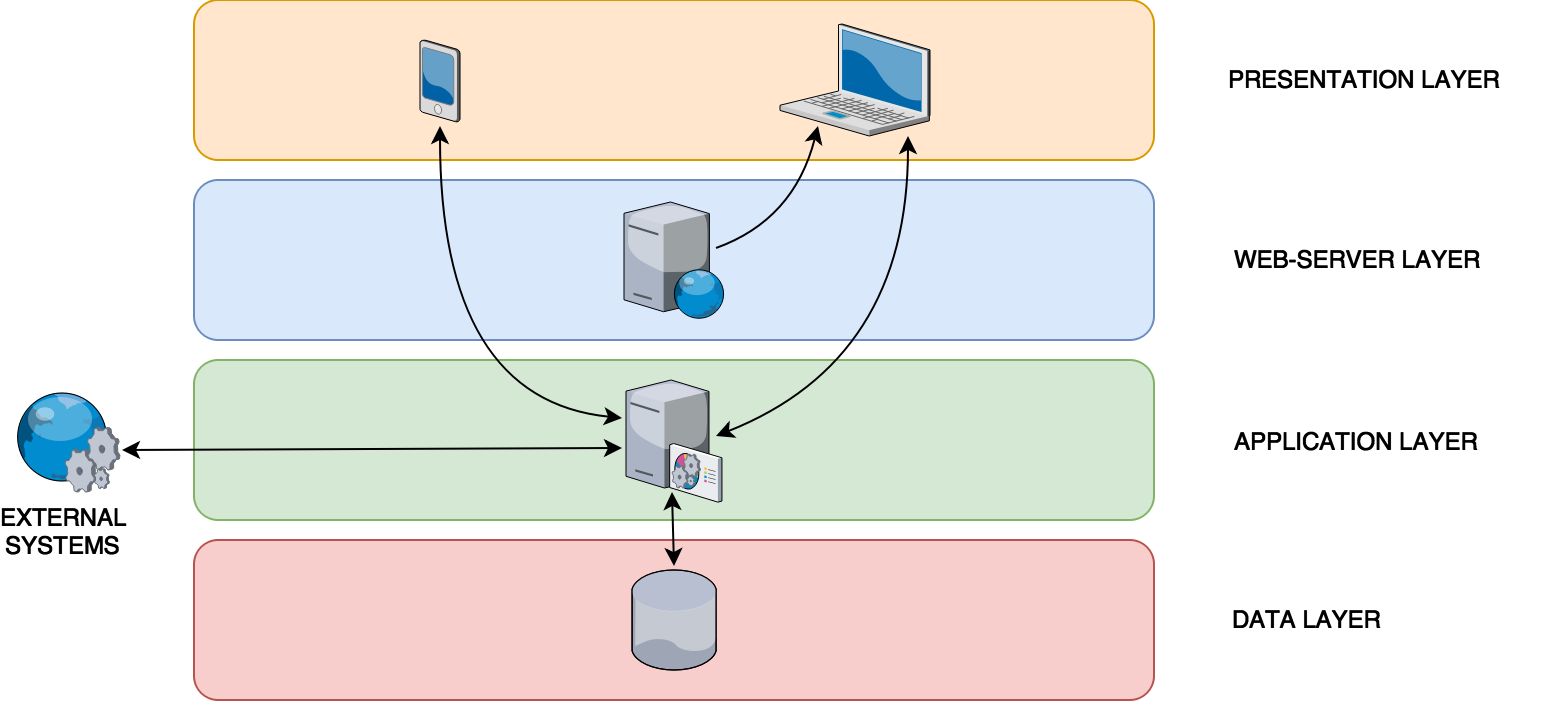
\includegraphics[width=0.95\textwidth]{img/diagrams/layers.png}
	\caption{Layer structure of the system.}
	\end{figure}

	\begin{figure}[ht]
	\centering
	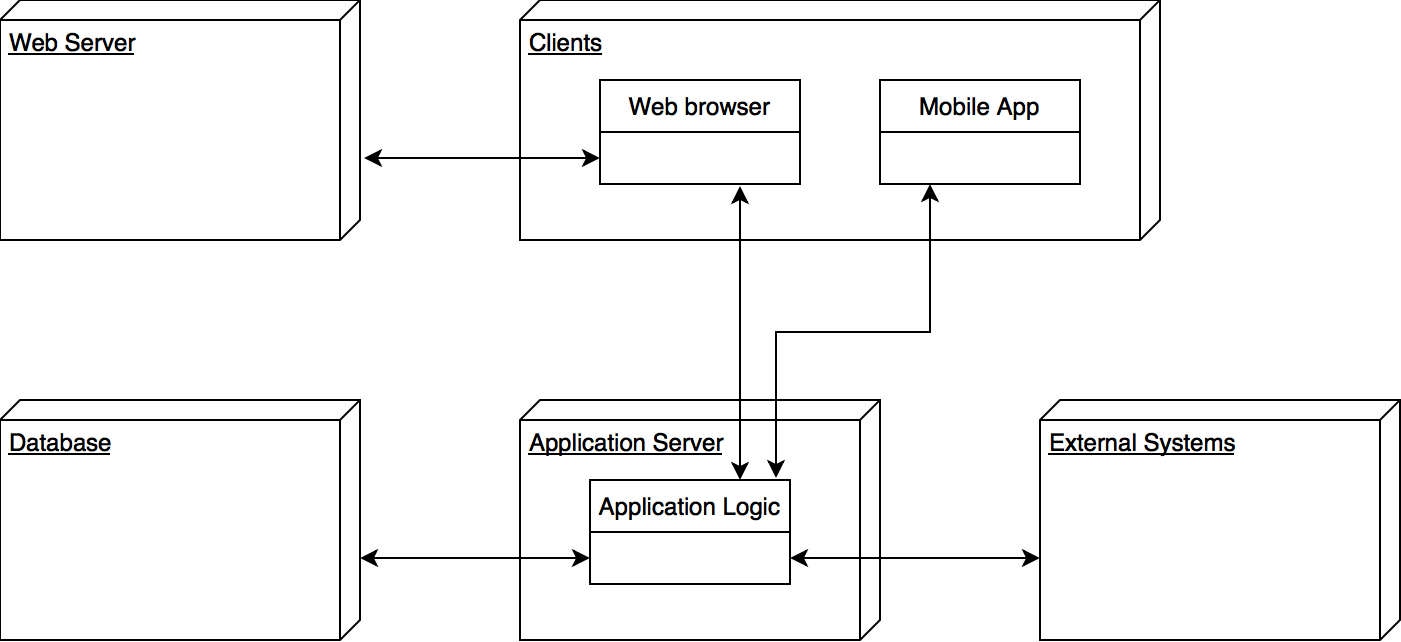
\includegraphics[width=0.75\textwidth]{img/diagrams/hlc.png}
	\caption{High-level components of the system.}
	\end{figure}

	\newpage

	\subsection{Component view}

	This section shows in a more detailed way the components introduced in the overview, their role and their interactions.

	\subsubsection{Database}
	The database layer must include a DBMS component in order to manage the insertion, modification, deletion, and registration of data transactions within the storage memory.
	
	The DBMS must guarantee the correct functioning of simultaneous transactions and ACID properties; the DBMS must be relational because the requirements of the application in terms of data storage do not require a more complex structure than the one provided by the relational data structure.
	
	The data layer must be accessible only through Application Server via a dedicated interface. The Application Server must provide a persistence unit to handle the dynamic behavior of all persistent application data.
	
	The database must be optimized during the implementation phase to ensure security by granting access to data according to the applicant's privilege level. Sensible data, for example passwords and personal information, must be encrypted correctly before being stored. Users must be granted access only on the provision of correct and valid credentials.

	\begin{figure}[ht]
	\centering
	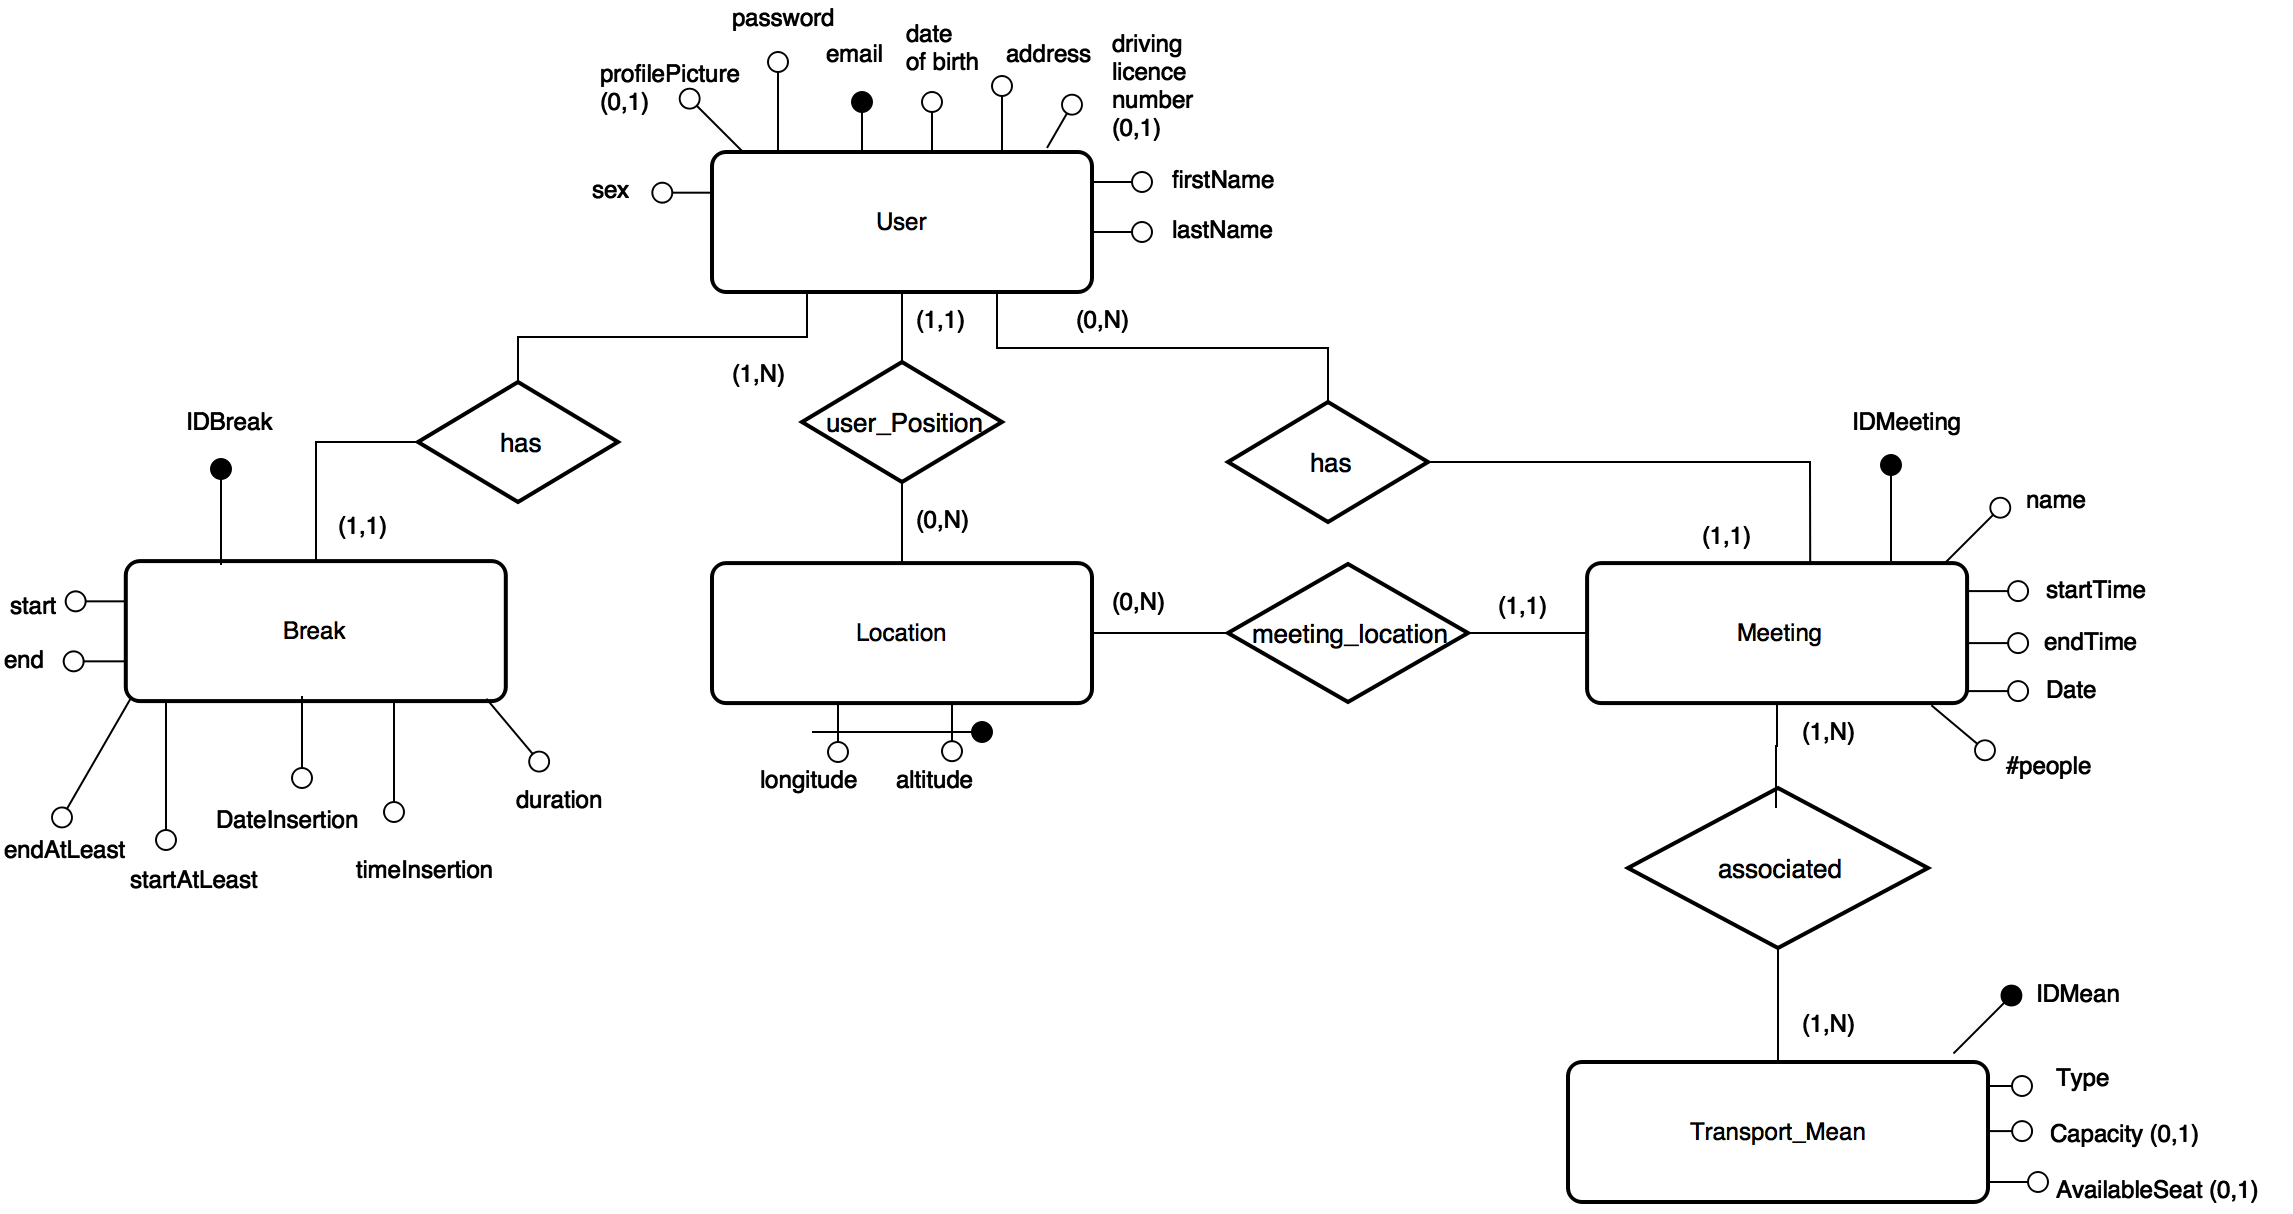
\includegraphics[width=\textwidth]{img/diagrams/er.png}
	\caption{ER Diagram.}
	\end{figure}


	\subsubsection{Application Server}
	This layer must handle business logic, data layer connections, and application access modes from different clients and external systems.
	
	The main feature of Application Server is the specific business logic modules that describe business rules and workflows for each feature provided by the application itself.
	
	The interface with the data layer must be managed by a dedicated persistence unit to ensure that only the Application Server can access the database.
	
	\bigskip
	Application Server must provide a means of interfacing with the Web server and mobile clients through specific APIs in order to separate the different levels from their individual implementation. It must provide a way to communicate with external systems by adapting the application to existing external infrastructures.
	
	\bigskip
	The main business logic modules must include:

	\begin{description}
	\item[UserManager:] This module must manage all the logics concerning to user account creation, login and management.
	\item[EventManager:] This module must contain all the logic needed to create and modify meetings and breaks. It must guarantee the consistency of the model preventing from overlapping among events. 
	\item[MapManager:] This module must contain all the logic used to locate users and meetings. 
	\item[TravelInformationProvider:] This module must be able to interface with external agents such as \textit{Travel information providers} (i.e., ATM, Trenord, Alitalia, etc.).
	\item[NotificationManager:] This module must be able to notify the user when it is necessary to do so (e.g. an user tries to insert a meeting that overlaps with a previous one).
	\end{description}


	\subsubsection{Web Server}
	The Web Server Layer is responsible to provide the web pages to the users that intends to access the application's services via web.
	
	\bigskip
	This layer does not contain any application logic; it only provides static web pages that, through propers Javascript scripts, are able to access the REST APIs of the Application Server and make it accessible to end users.

	\bigskip
	The scripts must be able to consume all the API's endpoints for the functionalities intended to be accessible via web.
	The communication with the APIs must be through textual data files over HTTPS (e.g. XML or JSON), as previously specified in \textit{Application Server} section.


	\subsubsection{Mobile Application Client}
	The Mobile Application Client must be designed to allow easy communication and implementation independent with the Application Server.
	The mobile application user interface should be designed following the guidelines provided by Android and iOS producers.
	The application must provide a software module that manages the GPS connection so that it can track location data by providing it to application servers.


	\subsubsection{Web Application Client}
	A \textit{Web Application Client} is any modern browser (eg., IE, Firefox, Chrome, Safari) able to run Javascript to allow the pages to consume the REST APIs of the \textit{Application Server}.


	\subsection{Deployment view}


	\subsection{Runtime view}


	\subsection{Component interfaces}
	
	
	\subsection{Architectural styles and patterns}


	\subsection{Other design decisions}


	\section{Algorithm Design}


	\section{User Interface Design}


	\subsection{UX diagrams}


	\subsection{User interface}


	\subsubsection{Web interface}


	\subsubsection{Mobile interface}


	\section{Requirements Traceability}


	\subsection{Functional requirements}


	\subsection{Non-functional requirements}


	\section{Implementation, Integration and Test Plan}


	\subsection{Entry criteria}


	\subsection{Elements to be integrated}


	\subsection{Integration testing strategy}


	\subsection{Sequence of components/Function integration}


	\subsubsection{Software integration sequence}


	\subsubsection{Subsystem integration sequence}


	\newpage
	\appendix
	\section{Appendix}


	\subsection{Software and tools used}

	The software and tools used during the drawing of this document are:

	\begin{description}
	\item[LaTex:] used to build this document.
	\item[Google Drive / Google Documents:] used to always update and share the documents.
	\item[draw.io:] used to draw diagrams (https://www.draw.io).
	\item[Marvel:] used to build the mockups (https://marvelapp.com).
	\item[GitHub:] used as version control and to keep it shared between group members and teachers (https://www.github.com).
	\end{description}
	

	\subsection{Hours of work}

	Most of the work on this document was made in the presence of both members of the group. The approximate number of hours worked by each member of the group is as follow (including hours spent in group work):
	
	\bigskip
	Davide Rossetto: about ... hours
	
	Alessandro Tatti: about ... hours

	
	\section{Bibliography}
	
	\begin{description}
	\item[[1{]}] AA 2017/2018 Software Engineering 2 - Requirements Analysis and Specification Document - Davide Rossetto, Alessandro Tatti
	\item[[2{]}] AA 2017/2018 Software Engineering 2 - Project goal, schedule and rules
	\item[[3{]}] IEEE Standard 1016:2009 System design - Software design descriptions
	\item[[4{]}]
	\end{description}

\end{document}
